% \subsection{Case Study: \sys-FaaS}
\subsection{Case Study: Serverless Computing (FaaS)}
\label{s:case-FaaS}

Recent works~\cite{10.1145/3472883.3486972, 10.1145/3503222.3507732, copik2022rfaas, wei2022provisioned} have tried to explore heterogeneous devices (e.g., DPU) for serverless to achieve better scalability and performance, e.g., Molecule~\cite{10.1145/3503222.3507732}. % (Fig.~\ref{fig:case-wingman-faas-arch}-a).
However, they usually require non-trivial modifications to both the serverless runtime and applications.

\myparagraph{\sys-FaaS.}
\sys supports serverless computing on CPU-DPU computers without modifying binaries of functions, language runtimes, and serverless runtime (Fig.\ref{fig:intro-wingman}-e).
Unlike Molecule which utilizes one serverless runtime to manage both CPU and DPU, \faas takes different PUs as standalone devices, but incorporating the \os to achieve efficient communication between functions transparently.
As Molecule's function are single-container sandboxes, \faas does not apply the \giptable.


% \myparagraph{Implementation.}
We implement \faas based on the Molecule's open-sourced homogeneous implementation, and utilizes its modified runc which support container fork for low latency startup.
\faas will preload \os for each function instance, but configure a \emph{configuration file} to only enable \gsocket between instances in the same function chain, i.e., one-function applications will not utilize \os.
\faas assumes the global gateway will schedule a function chain in a one heterogeneous computers.
We compare \faas with Molecule and Molecule-homo (a homogeneous version for CPU-only computer).



\begin{figure}[t]
 \setlength{\belowcaptionskip}{-10pt}
 \setlength{\abovecaptionskip}{0pt}
  \begin{minipage}{0.49\linewidth}
    \centering 
    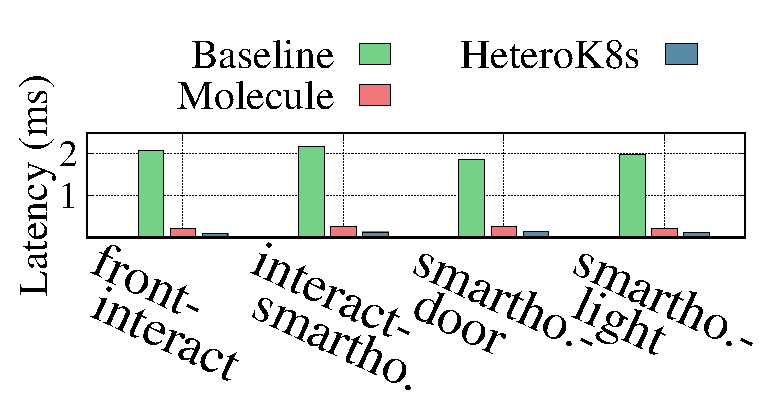
\includegraphics[width=1\linewidth]{figs-eval/eval-runtime-micro-dag-host-host.eps}
    \footnotesize
    \textbf{(a) CPU to CPU}
  \end{minipage}
  \begin{minipage}{0.49\linewidth}
    \centering 
    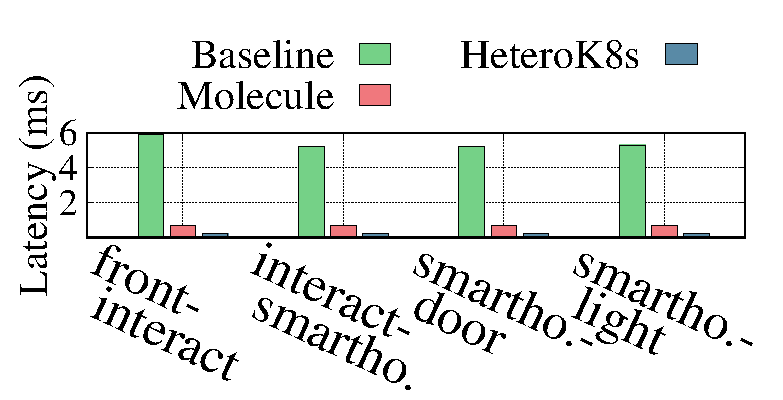
\includegraphics[width=1\linewidth]{figs-eval/eval-runtime-micro-dag-NIC-NIC.eps}
    \footnotesize
    \textbf{(b) DPU to DPU}
  \end{minipage}

  \begin{minipage}{0.49\linewidth}
    \centering 
    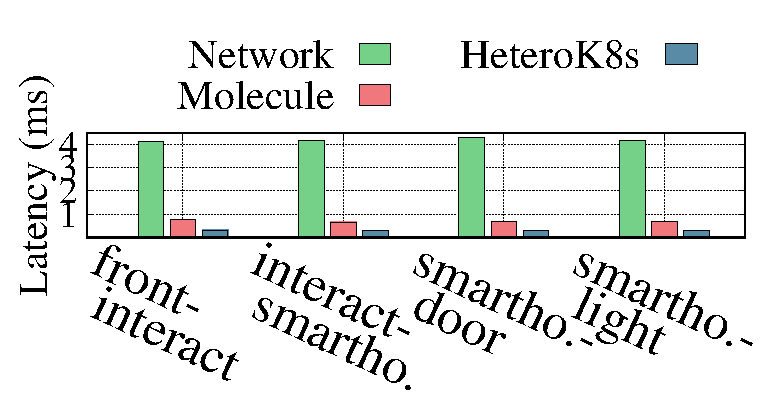
\includegraphics[width=1\linewidth]{figs-eval/eval-runtime-micro-dag-host-NIC.eps}
    \footnotesize
    \textbf{(c) CPU to DPU}
  \end{minipage}
  \begin{minipage}{0.49\linewidth}
    \centering 
    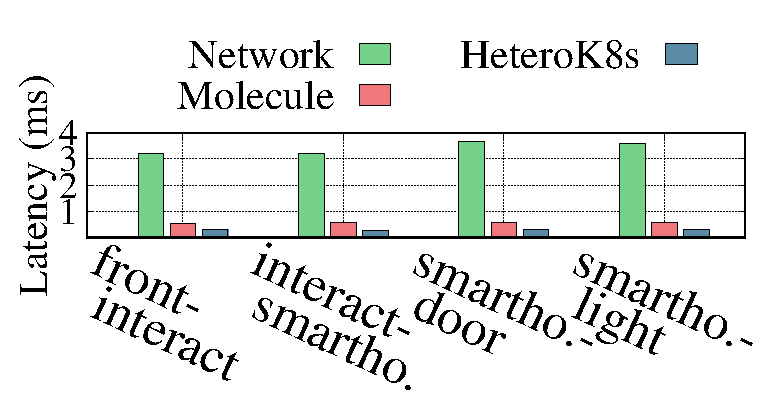
\includegraphics[width=1\linewidth]{figs-eval/eval-runtime-micro-dag-NIC-host.eps}
    \footnotesize
    \textbf{(d) DPU to CPU}
  \end{minipage}
  \caption{\textbf{Serverless DAG communication latency.} \textit{\faas achieves 2x lower latency compared with state-of-the-art system, Molecule.}}
  \label{fig:eval-runtime-micro-dag}
\end{figure}



\myparagraph{Microbenchmarks.}
We perform microbenchmarks to analyze the communication latency between two functions in a chain.
We take Alexa skills~\cite{socc20-serverlessbench} as an example,
and compare \faas with Molecule (using nIPC) and the baseline (Molecule's homogeneous version using Node.js Express).
% to evaluate DAG communication latency.
We consider four cases, including CPU-only, DPU-only, CPU-to-DPU and DPU-to-CPU.
The results are shown in Fig.\ref{fig:eval-runtime-micro-dag}.
Molecule already achieves about 10x lower latency compared with the Baseline because of its efficient nIPC-based communication.
\faas can achieve even better performance (about 2x) because Molecule requires one additional IPC call to invoke the Hetero-Shim.
The results of Molecule is better than the reported data~\cite{10.1145/3503222.3507732} because of the better hardware settings in our environment.




\begin{figure}[t]
\setlength{\belowcaptionskip}{-10pt}
\setlength{\abovecaptionskip}{0pt}
\begin{minipage}[t]{0.66\linewidth}
  \centering 
  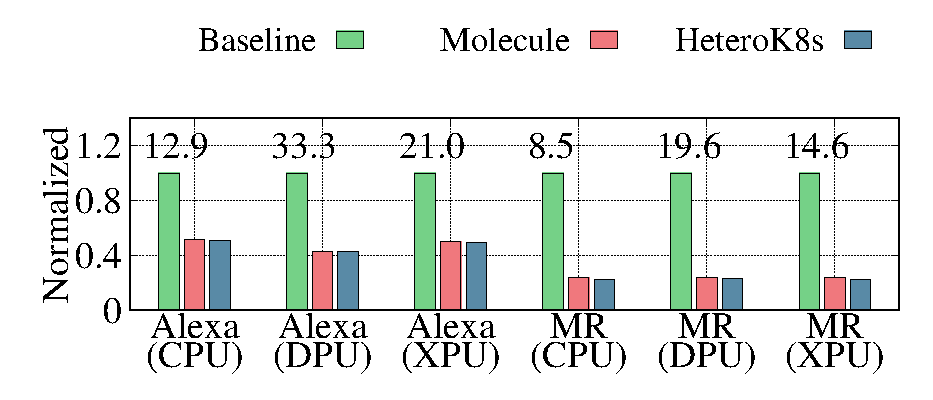
\includegraphics[width=1\linewidth]{figs-eval/eval-apps-chain.eps}
  \footnotesize    
\textbf{(a) Apps on Bluefield-2}
\end{minipage}  
\begin{minipage}[t]{0.33\linewidth}
  \centering 
  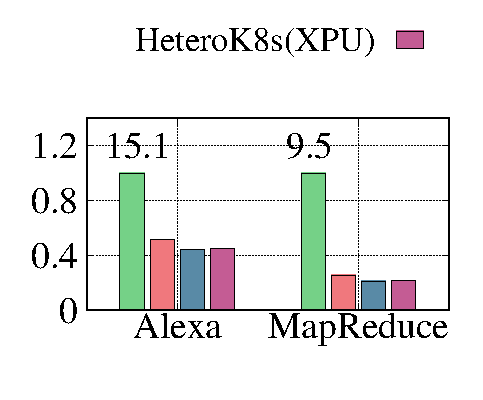
\includegraphics[width=1\linewidth]{figs-eval/eval-apps-chain-cxl.eps}
  \footnotesize    
\textbf{(b) Apps on CXL-DPU}
\end{minipage}  
\caption{\textbf{Chained Applications.}
	\textit{MR for MapReduce. XPU for Cross-PU.}
	}
  \label{fig:eval-faas-dag-apps}
\end{figure}

\myparagraph{Applications.}
We analyze end-to-end latency of two chained applications from ServerlessBench and FunctionBench, Alexa and MapReduce.
Alexa comprises five Node.js functions and MapReduce includes three Python functions.
We compare three systems, Baseline (i.e., Molecule-homo), Molecule, and \faas under three cases, CPU, DPU and cross-PU.
In the case of cross-PU, we ensure that all inter-function calls are cross PU, e.g., in Alexa, the 1st, 3rd, and 5th functions are in the host CPU, and the 2nd and 4th functions are in the DPU.
All the instances are warm-boot (without cold startup costs).
The results are shown in Fig.\ref{fig:eval-faas-dag-apps}.
Molecule can achieve 1.94--2.32x less end-to-end latency in Alexa and 4.20--4.21x less latency in MapReduce,
while \faas can achieve better latency, achieving 1.96--2.34x less end-to-end latency in Alexa and 4.19--4.45x less latency in MapReduce compared with the baseline.

